\documentclass{beamer}
\usetheme{greeniot}
\usepackage[utf8]{inputenc}
\usepackage{hyperref}
\usepackage{pgf}
\usepackage{tikz}
\usepackage{amsmath}
\usepackage{amsfonts}
\usepackage{amssymb}
\usepackage{graphicx}
\usetikzlibrary{calc}
\usetikzlibrary{positioning}
\usetikzlibrary{arrows.meta}

\hypersetup{%
	pdftitle={From Ethernet to InfiniBand},
	pdfauthor={Author},
	pdfsubject={Sommerakademie der Studienstiftung, Leysin, 2016},
	pdfcreator=pdflatex,
	pdfproducer=pdflatex,
	pdfnewwindow=true,
	pdfpagemode=FullScreen,
	pdfview=FitBH,
	plainpages=false,
	baseurl={./}
}

% Title Page
\title[From Ethernet to InfiniBand]{%
	\Large From Ethernet to InfiniBand\\
	[5mm] \normalsize Sommerakademie in Leysin\\
	AG 2 -- Effizientes Rechnen
}
\author[Philipp Czerner]{Philipp Czerner}
\institute[]{%
	TU Clausthal\\[3mm]
}
\date{August 2016}
\titlegraphic{%
	\vspace{5mm}%
	
\includegraphics[height=1.5cm]{logo_sdv.pdf}%
}


\begin{document}

\begin{frame}
	\titlepage
\end{frame}

\begin{frame}
	\frametitle{Outline}
	\tableofcontents
\end{frame}

\AtBeginSection[]{%
	\begin{frame}
		\tableofcontents[currentsection]
	\end{frame}
}

\section{OSI Model}

\begin{frame}{OSI Model}
\begin{itemize}
	\item Open Systems Interconnection model
	\item Describes and standardises the workings of a communications system
	\item Partitions into layers 1-7
	\begin{itemize}	
		\item Each layer uses the functionionality of the layer below and provides an interface for the one above
		\item Direct communication only happens on layer 1 (Physical layer)
	\end{itemize}
\end{itemize}
\begin{center}
	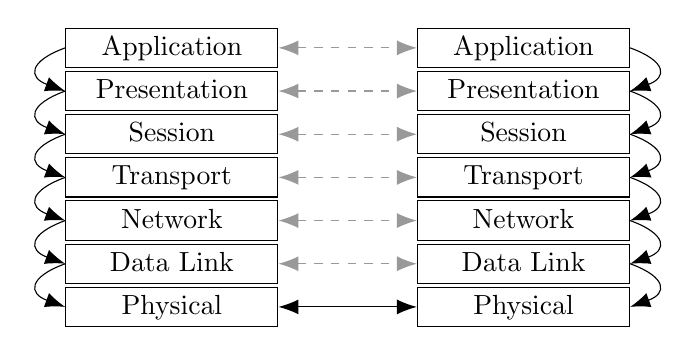
\begin{tikzpicture}[scale=0.5,node distance=1pt,<->/.tip={Latex[scale=1.5]}]
	\tikzstyle{box}=[rectangle,align=center,draw,text height=1.5ex
		,text depth=.25ex,text width=7em]
	\tikzstyle{dashy}=[<->,dashed,color=black!40]
	
	\node[box] (n1) at (0,0) {Physical};
	\node[box] (m1) [right=5em of n1] {Physical};
	\foreach \x/\xx/\y in {2/1/Data Link,3/2/Network,4/3/Transport,5/4/Session,6/5/Presentation,7/6/Application} {
	\node[box] (n\x) [above=of n\xx] {\y};\node[box] (m\x) [above=of m\xx] {\y};}
	
	\draw[<->] (n1) -- (m1);
	\foreach \x/\y in {2/1,3/2,4/3,5/4,6/5,7/6} {\draw[dashy] (n\x ) -- (m\x );
	\draw[<-] (n\y.west) ..controls +(160:1cm) and +(200:1cm).. (n\x.west);
	\draw[<-] (m\y.east) ..controls +(20:1cm) and +(340:1cm).. (m\x.east);}
	
	\end{tikzpicture}
\end{center}
\end{frame}


\begin{frame}{OSI Model – Layers 1 to 4}
\begin{itemize}
	\item Layer 1 (Physical) deals with the specification of the physical medium (pin layout, timing, half/full duplex)
	\begin{itemize}
		\item Examples: Ethernet physical layer, DSL, SONET/SDH
	\end{itemize}
	\item Layer 2 (Data Link) allows to transfer data reliably between neighbouring nodes (flow control, error checking, connections)
	\begin{itemize}
		\item Examples: Ethernet, PPP, ATM
	\end{itemize}
	\item Layer 3 (Network) handles multi-node networking (address translation, routing, traffic control)
	\begin{itemize}
		\item Examples: IPv4, IPv6
	\end{itemize}
	\item Layer 4 (Transport) provides a reliable data transfer between nodes in the network (acknowledging, error control, sequence numbers)
	\begin{itemize}
		\item Examples: TCP, UDP
	\end{itemize}
\end{itemize}
\end{frame}

\section{Ethernet}

\begin{frame}{Ethernet}
\begin{itemize}
	\item Ethernet is a family of standards, mostly for LANs
	\item 10BASE-T, 100BASE-TX and 1000BASE-T are commonly used in consumer hardware, using shielded twisted pair cabling
	\item Ethernet is located at both the physical layer and the data link layer
	\begin{itemize}
		\item It does not provide all functions the OSI model specifies, for example there is no error recovery
	\end{itemize}
	\item Recent standards have raised the possible data rate to about 100 Gbit/s
\end{itemize}
\end{frame}

\begin{frame}{Ethernet – 100BASE-TX}
\begin{itemize}
	\item Most common form of LAN technology in consumer hardware
	\item Uses a category 5 (or better) twisted pair cable and an 8P8C plug (sometimes called RJ45)
	\begin{itemize}	
		\item Only two of the four pairs of a standard Cat-5 cable are used
	\end{itemize}
	\item Bit rate of 100 Mbit/s
\end{itemize}
\end{frame}

\begin{frame}{Ethernet – Gigabit and beyond}
\begin{itemize}
	\item Gigabit, 10G and 40G Ethernet continue to evolve the Ethernet family
	\item As of June 2016 44\% of the Top500 computers use an Ethernet type interconnect (41\% use Infiniband), making it the most used interconnect
\end{itemize}
\end{frame}


\section{InfiniBand}

\begin{frame}{InfiniBand}
\begin{itemize}
	\item InfiniBand (IB) is a networking technology with a focus an high bandwidth and low latency
	\item Like Ethernet there are multiple standards
	\item Used in High-Performance-Computing
	\item Resides at layers 1-4 of the OSI model
	\item Standard protocols (like TCP/IP) can be mapped
	\item Throughoutput of up to 97 Gbit/s for a 4X link
	\begin{itemize}
		\item The earliest version (in 2001) already had 8 Gbit/s
	\end{itemize}
\end{itemize}
\end{frame}

\begin{frame}{RDMA}
	\begin{itemize}
		\item Traditionally the OS copies application data into buffers prior to sending
		\item Remote Direct Memory Access (RDMA) enables a zero-copy transfer
		\item The HCA of the remote node directly accesses the application memory
		\begin{itemize}	
			\item Does not involve the remote CPU, OS or caches
			\item No context switches on either end
		\end{itemize}
		\item The application must register the memory ranges with the HCA beforehand via the Kernel
		\begin{itemize}	
			\item The registration returns a key to the memory needed to access it remotely, for security reasons
		\end{itemize}
		
	\end{itemize}
\end{frame}

\begin{frame}{InfiniBand – Architecture}
\begin{itemize}
	\item A host channel adapter (HCA) connects a CPU to the IB network over a PCI Express interface
	\item The HCA provides functionality of layers 1-4 in hardware
	\item Provides both send/recieve and RDMA based communication
	\item Uses a queue based model, consisting of a \textit{Queue Pair} (QP) with a send and a recieve queue
	\begin{itemize}	
		\item \textit{Work Queue Requests} (WQR) are placed in either of these
		\item WQR can specify a send/recieve or RDMA request
	\end{itemize}
	\item Both reliable and unreliable communication is available
\end{itemize}
\end{frame}

\begin{frame}{InfiniBand – Key Advantages}
\begin{itemize}
	\item Transmitting data bypasses the kernel in order to reduce latency
	\begin{itemize}	
		\item The kernel is involved in things like registering memory or initializing the HCA, which are not time sensitive
	\end{itemize}
	\item Remote Direct Memory Access (RDMA) allows one-sided communication
\end{itemize}
\end{frame}

\begin{frame}{InfiniBand – Power Consumption}
\begin{itemize}
	\item Implementing the network stack in hardware reduces CPU overhead
	\item RDMA also lowers CPU involvement
	\item 48\% of the top 100 of the Green500 (June 2016) use Infiniband, 17\% use Ethernet (vs. 41\% and 44\% for the Top500, respectively)
	\item On some HPC systems the interconnect consumes 15-20\% of the total power
	\begin{itemize}
		\item The percentage increases when the system is not at full load
	\end{itemize}
\end{itemize}
\end{frame}


%\begin{frame}{InfiniBand}
%	\begin{itemize}
%		\item InfiniBand (IB) is a networking technology 
%	\end{itemize}
%\end{frame}

\end{document}
